\begin{frame}[fragile]
  \frametitle{Colecciones}

  \begin{enumerate}[3.]
    \item Diccionarios    
  \end{enumerate}

  Los diccionarios deben su nombre a que son colecciones que relacionan una clave y un valor. El primer valor se trata de la clave y el segundo del valor asociado a la clave. La diferencia principal entre los diccionarios y las listas o las tuplas es que se accede a su valor por medio de su clave usando corchetes.

  \begin{itemize}
    \item Ejemplo:
  \end{itemize}

  \begin{figure}
    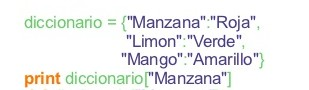
\includegraphics[width=0.6\textwidth]{Imagenes/Diccionarios.jpg}
    \caption{\label{fig:Ejemplo3}Creaci\'on de un diccionario en Python.}
  \end{figure}  
 
 
\end{frame}
